\documentclass[thesis.tex]{subfiles}
\begin{document}

\chapter{SpeedCam}\label{chap:basics}

This chapter will describe the three following parts. At first it will outline the general idea of the SpeedCam approach for any network type. After this it will describe the specific adaptation for the SCION network. At last there will be an explanation what has to be changed for SCIONLab and the reason for that.

\section{Overview}
SpeedCam is an heuristic approach to monitor network traffic with regards to limited resources. It analyses the network structure and decided based on the heuristic where are good places to monitor local traffic. The approach also tries to reduce the necessary amount of probes to minimize the resource impact an the machines.


\subsection{Inspection game}
The idea behind SpeedCam is based on the \textit{Inspection Game} in the game theory \todo{Quelle einfügen}. Inside the game is a \textit{task} to be done under defined \textit{rules}. The execution of the task can be simpler, more efficient or more effective with a violation of these rules. The task is performed by one of the two parties, the \textit{inspectee} and the compliance of the rules costs resources and is monitored by the second party, the \textit{inspector}. The inspectee has a general interest to break the rules to perform better, while the inspector wants to reduce his amount of inspections to use as few as possible resources. The possible combination are shown in \autoref{tab:inspectionGameMatrix}.

\begin{table}[h]
    \centering
    \begin{tabular}{cc|c|c|}
        & \multicolumn{1}{c}{} & \multicolumn{2}{c}{Inspector}\\
        & \multicolumn{1}{c}{} & \multicolumn{1}{c}{Inspect}  & \multicolumn{1}{c}{Ignore} \\\cline{3-4}
        \multirow{2}*{Inspectee}  & Comply & $A$ & $C$ \\\cline{3-4}
        & Violate & $B$ & $D$ \\\cline{3-4}
    \end{tabular}
    \caption{Inspection game matrix.}
    \label{tab:inspectionGameMatrix}
\end{table}

The cases $B$ and $C$ are good investments of the inspectors limited resources. In the first one he didn't inspect while the task was performed without violation and in the second one the inspector found the culprit. For case $A$ were the resources of the inspector wasted because there was no reason to inspect. The inspector failed in its task in case $D$, because he missed a violation of the rules by not investing the resources.

Because of the shown cases and it results it is obvious that a \textit{pure strategy} doesn't make sense in this game. When the inspector always inspect he will waste resources and when the inspector always ignores he fails his task. Instead of a pure strategy there must exist a \textit{mixed strategy} defined by probabilities for each action to be chosen. \todo{Quelel für Nash Beweis}.


\subsection {Generalized concept}
The previously described form of the Inspection game is adopted for networks for this work. The \textit{nodes} of a network are the \textit{inspectees}, their \textit{task} is to \textit{transfer} many data in a short time. The \textit{rule} for all nodes is, that a transaction of data \textit{mustn't exceed the link limits} or disturb other nodes transfer. These limits can be given by the physical cable nature or are artificial bilateral agreed limits. A \textit{detected violation} of these rules can result in throttling the bandwidth or even exclude the node from the node, temporary or permanently. A node can try to exceed the limits and so breaking the rule, while avoiding any inspection. 

The \textit{inspector} in such a game has the possibility to monitor a nodes network traffic. Monitoring a node costs computation resources such as memory or cpu cycles\todo{Quelle für Leistungsaufwand von switches nur für switching}. Both can be critical for a switch to send packets. Therefore an inspection, necessary or not, will have an impact on the network throughput. The challenge of the inspector is to only monitor when a node is exceeding its limits. He will be presented in this work as the SpeedCam approach. These will give the inspector an heuristic with the goal to increase the amount of cases for $B$ and $C$ and to reduce it for $A$ (not wasting resources) and $D$ (fairness for network member).

The general concept of SpeedCam applies to types of networks which meet the following requirements. The network must consist of \textit{nodes}, ASes, and \textit{links}, which connect only two ASes. The nodes and links must form an undirected graph. For SpeedCam it is not necessary that the graph must be known in the first place nor to be static. This is important because real networks tend to be dynamic and to be decentralized with only partial knowledge about its structure. The inspector must have access to these network in such a form, that he can gain knowledge about the networks structure and monitor a nodes traffic.

When the requirements are met the inspector can be run as a component. He executes the SpeedCam approach and stores the necessary information about the nodes. It is described in this work as a centralized component, but it can be split into multiple inspectors each responsible for a subnetwork. 

The SpeedCam approach consists of the following four phases:
\todo{use graphic instead of list}
\begin{easylist}
    \MyNumberedListProperties
    \ListProperties(Start1=0)
    # Exploration
    # Selection
    # Monitoring
    # Conclusion
\end{easylist}

The exploration phase is the 0-th phase because it can be skipped if the network is static and fully explored. This phase can also be running in the background in parallel to the other phases. Phase 1 to 3 must be running in sequential order, because they depend on each other results. The next sections will explain each phase in detail.

\subsection{Exploration}
This phase has the goal to create an undirected graph of the network to monitor. The structure of the network is necessary for the following phases. 

For the general concept of the SpeedCam approach exists multiple possibilities to explore the underlying network. Because the only assumption about the network is that nodes are connected via links these possibilities are also general and has some flaws. In later discussed specialized forms of the SpeedCam approach there are fewer flaws.

The first possibility is to manually create the graph. A network, virtual or physically present, must be created by an entity, be it a humanoid administrator or a program. Every change of the network can be logged and used to create the graph. This is obviously a tedious task and not error prone. 

Another possibility needs a start point inside the network. With such a start point it is possible to get all connected nodes with the use of a traversal algorithm, like Breadth-First, Depth-First, Djikstra or Floyd–Warshall. This is for example used by the Border-Gateway-Protocol (BGO).\todo{Quellen für alles}. This is for such a general network the way to explore the network graph.

The exploration phase itself needs to be constantly repeated to react to changes inside the network. Inactive or disconnected nodes doesn't need to be monitored.

\subsection{Selection}

Based on the results of the previous exploration phase, the selection phase uses the network information to select good candidates for probe points.

\section{Detection scheme}
This part will contain the description about the detection scheme. It will outline how to detect a greedy user and provide a detailed overview of its functionality.

\subsection{Basic idea}
The task of the detection scheme is to identify a greedy AS inside an ISD using multi-path connections. 

A central unit inside the ISD will be able to start an inspection and inspect ASes bandwidth usage. This is done by a core AS, which is called \textbf{inspector}. 

The inspector will randomly choose ASes inside its ISD to measure the bandwidth. The chosen ASes are called \textbf{speed cam}. They will collect for a certain amount of time the metrics and aggregate them over time. When the duration is to end, the speed cams will sent the data to the inspector.

When the inspector received the data of all speed cams, he will decide, which user is greedy and who are not. The decision process will be explained in later parts of this work.


\begin{figure}[h]
    \begin{subfigure}{.32\linewidth}
        \centering
        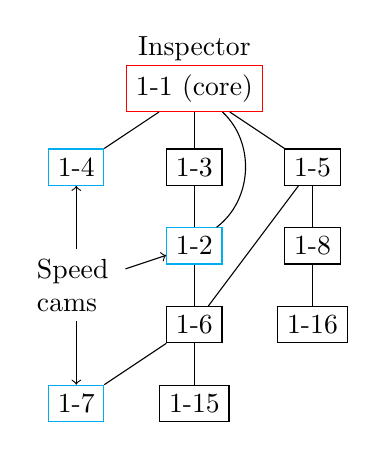
\begin{tikzpicture}
        \node (inspector) at (0, 0.5) {Inspector};
        \node[shape=rectangle,draw=red] (1-1) at (0,0) {1-1 (core)};
        \node[shape=rectangle,draw=cyan] (1-2) at (0,-2) {1-2};
        \node[shape=rectangle,draw=black] (1-3) at (0,-1) {1-3};
        \node[shape=rectangle,draw=cyan] (1-4) at (-1.5,-1) {1-4};
        \node[shape=rectangle,draw=black] (1-5) at (1.5,-1) {1-5};
        \node[shape=rectangle,draw=black] (1-6) at (0,-3) {1-6};
        \node[shape=rectangle,draw=cyan] (1-7) at (-1.5,-4) {1-7};
        \node[shape=rectangle,draw=black] (1-8) at (1.5,-2) {1-8};
        \node[shape=rectangle,draw=black] (1-15) at (0,-4) {1-15};
        \node[shape=rectangle,draw=black] (1-16) at (1.5,-3) {1-16};
        \node (speedcam) at (-1.5, -2.5) [text width=1cm]{Speed cams};        
        
        \path[-]	
        (1-1) edge (1-4)
        (1-1) edge (1-3)
        (1-1) edge (1-5)
        (1-1) edge[bend left=50] (1-2)
        (1-2) edge (1-6)
        (1-3) edge (1-2)
        (1-5) edge (1-8)
        (1-5) edge (1-6)
        (1-6) edge (1-7)
        (1-6) edge (1-15)
        (1-8) edge (1-16)
        ;
        
        \path[->]
        (speedcam) edge (1-4)
        (speedcam) edge (1-2)
        (speedcam) edge (1-7);
        \end{tikzpicture}
        \caption{Inspector choose ASes for speed cams}
        \label{fig:main:exampleDetectionSchemeSub1}
    \end{subfigure}%
    \begin{subfigure}{.32\linewidth}
        \centering
        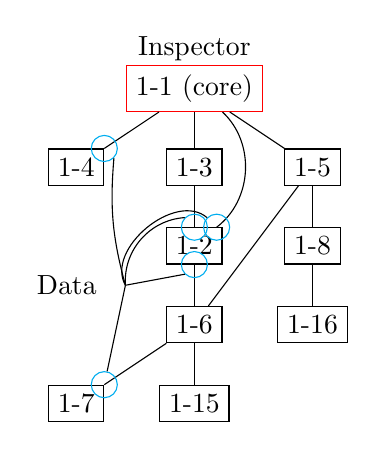
\begin{tikzpicture}
        \node (inspector) at (0, 0.5) {Inspector};
        \node[shape=rectangle,draw=red] (1-1) at (0,0) {1-1 (core)};
        \node[shape=rectangle,draw=black] (1-2) at (0,-2) {1-2};
        \node[shape=rectangle,draw=black] (1-3) at (0,-1) {1-3};
        \node[shape=rectangle,draw=black] (1-4) at (-1.5,-1) {1-4};
        \node[shape=rectangle,draw=black] (1-5) at (1.5,-1) {1-5};
        \node[shape=rectangle,draw=black] (1-6) at (0,-3) {1-6};
        \node[shape=rectangle,draw=black] (1-7) at (-1.5,-4) {1-7};
        \node[shape=rectangle,draw=black] (1-8) at (1.5,-2) {1-8};
        \node[shape=rectangle,draw=black] (1-15) at (0,-4) {1-15};
        \node[shape=rectangle,draw=black] (1-16) at (1.5,-3) {1-16};
        \node (data) at (-1.5, -2.5) [text width=1cm]{Data};
        
        \path[-]		
        (1-1) edge node[shape=circle,draw=cyan, at end] (data1) {} (1-4)    
        (1-1) edge (1-3)
        (1-1) edge (1-5)
        (1-1) edge[bend left=50] node[shape=circle,draw=cyan, at end] (data2) {} (1-2)
        (1-2) edge node[shape=circle,draw=cyan, at start] (data3) {} (1-6)
        (1-3) edge node[shape=circle,draw=cyan, at end] (data4) {} (1-2)
        (1-5) edge (1-8)
        (1-5) edge (1-6)
        (1-6) edge node[shape=circle,draw=cyan, at end] (data5) {} (1-7)
        (1-6) edge (1-15)
        (1-8) edge (1-16)
        ;
        \path[-]
        (data1.south east) edge[bend right=10] (data.east)
        (data2.north west) edge[bend right=80] (data.east)
        (data3.south west) edge (data.east)
        (data4.north west) edge[bend right=45] (data.east)
        (data5) edge (data.east)
        ;
        \end{tikzpicture}
        \caption{Speed cams collect data about traffic}
        \label{fig:main:exampleDetectionSchemeSub2}
    \end{subfigure}%
    \begin{subfigure}{0.32\linewidth}
        \centering
        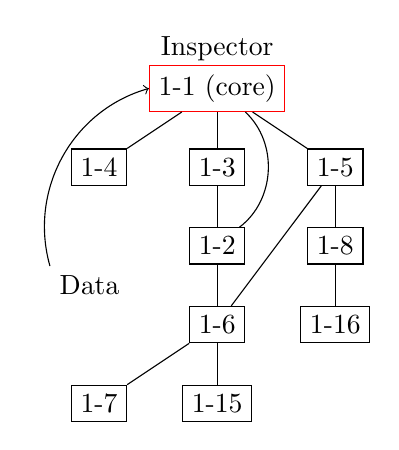
\begin{tikzpicture}
        \node (inspector) at (0, 0.5) {Inspector};
        \node[shape=rectangle,draw=red] (1-1) at (0,0) {1-1 (core)};
        \node[shape=rectangle,draw=black] (1-2) at (0,-2) {1-2};
        \node[shape=rectangle,draw=black] (1-3) at (0,-1) {1-3};
        \node[shape=rectangle,draw=black] (1-4) at (-1.5,-1) {1-4};
        \node[shape=rectangle,draw=black] (1-5) at (1.5,-1) {1-5};
        \node[shape=rectangle,draw=black] (1-6) at (0,-3) {1-6};
        \node[shape=rectangle,draw=black] (1-7) at (-1.5,-4) {1-7};
        \node[shape=rectangle,draw=black] (1-8) at (1.5,-2) {1-8};
        \node[shape=rectangle,draw=black] (1-15) at (0,-4) {1-15};
        \node[shape=rectangle,draw=black] (1-16) at (1.5,-3) {1-16};
        \node (data) at (-1.5, -2.5) [text width=1cm]{Data};
        
        \path[-]	
        (1-1) edge (1-4) 
        (1-1) edge (1-3)
        (1-1) edge (1-5)
        (1-1) edge[bend left=50] (1-2)
        (1-2) edge (1-6)
        (1-3) edge (1-2)
        (1-5) edge (1-8)
        (1-5) edge (1-6)
        (1-6) edge (1-7)
        (1-6) edge (1-15)
        (1-8) edge (1-16)
        ;
        
        \path[->]
        (data.north west) edge[bend left=45] (1-1.west);
        \end{tikzpicture}
        \caption{Speed cams report data to inspector}
        \label{fig:main:exampleDetectionSchemeSub3}
    \end{subfigure}
    \caption{Example of detection scheme}
    \label{fig:main:exampleDetectionScheme}
\end{figure}

The \autoref{fig:main:exampleDetectionScheme} shows an example for the detection scheme. It shows a the ISD 1 and its ASes. In \autoref{fig:main:exampleDetectionSchemeSub1} is the process of choosing speed cams visualized. The ASes 1-2, 1-4 and 1-7 are randomly chosen and now called speed cams. For a certain amount of time, the speed cams collect data about traffic through their border router. This can be seen in \autoref{fig:main:exampleDetectionSchemeSub2}. After the collection is finished, the data is sent to the inspector, which is shown by \autoref{fig:main:exampleDetectionSchemeSub3}.

The following section will explain the details about the selection, the data to collect and to classify the user.

\subsection{Selection process}
This part will explain the process how ASes are selected to be speed cams. It will outline what are the parameters and conditions to be selected and what are the results.

The selection of an AS as a speed cam is not trivial. It directly effects the accuracy and the efficiency of the measurement, which is a successor phase of the selection. Inactive ASes on the edge of the network represent a bad selection. They are incapable of monitoring the flow of data through the network, because they are not central enough. Also an inactive AS itself is probably not a greedy AS, while a busy AS can be the source of a congestion. A good selection has to achieve the opposite and result in a high accuracy.

The process of selection should not be predictable and so must be randomized. Each AS inside the network should have a chance to be picked. This makes it impossible for malicious and greedy ASes to predict the speed cam placements and the possibility to avoid them. They are not able to use unobserved paths to avoid the punishment. As described before a good selection is necessary for a high accuracy, the chances of ASes to be picked are higher if they are good candidates. But even very bad candidates have a small chance to be picked.

It is also important to pick as few ASes as possible for monitoring. The inspector can receive the complete network flow by monitoring all ASes inside it, but this is not efficient in sight of minimal performance impact and so not practical. The size should also be dynamic and scale with the amount of ASes in the network. A good start to be scalable is that the size of speed cams is $log(n)$, where $n$ is the size of ASes inside the network. To increase the unpredictability it is crucial to use a random interval instead of a fixed value. 

The next parts will explain in detail the different metrics and parameters important to the selection process.


\subsubsection{Selection criteria}

As described in the introduction of this section any AS has a chance to be selected as a SpeedCam. This part will list and describe each criteria important for the selection. They are divided in two categories, which are desribed later. The denotations of these criteria will later be used to present a calculation of the chance to be picked.
\todo{Maybe a visualization of a test graph?}

The following presented criteria are considered \textbf{static} and can be calculated without a history of past measurements. They only require the topology of the ISD.

\textbf{Degree} [ $deg(AS)$ ]: The sum of incoming and outgoing connection of an AS. The reason for assuming this criterion is that an AS with a high amount of connection represents a central node inside the network. This leads to the heuristic that a high degree has a bigger chance to record a great part of the networks traffic.

\textbf{Total capacity} [ $cap(AS)$ ]: The sum of the connection capacity of an AS. The capacity is the subscribed maximum possible bandwidth a connection can transfer. Similar to the \textbf{Degree} this criteria is to find central hubs inside a network. ASes with a high capacity will be often by other ASes to transfer their data, so this leads to a good possibility to measure the traffic at theses ASes.

The now following criteria are \textbf{dynamic} and requires a history of past measurements (episodes). The amount of entries can vary based on the needs of an ISD.

\textbf{Success rate} [ $SU_k(AS)$ ]: Any AS which was a SpeedCam in an episode $k$ episodes ago and when the source of congestion was identified is rewarded by a point and considered a successful SpeedCam. The opposites, not able to identify the source, are not rewarded and receive no points. This can be abstracted as a one (1) for a success in an episode and a zero (0) for a failure. A successful AS so will have a higher probability to be selected again than a unsuccessful AS. 
Considering the fact that a network is a dynamic element and traffic can vary it is important to weight the successes. This leads to the assumption, that a more recent episode is more important as an older one. The \textbf{success rate} of an AS for last-$k$ episodes is calculated as the following:

$$SU_{k}(AS) = \sum_{n=0}^{k} \frac{1}{n+1}*su_{k-n}(AS)$$

\textbf{Average activity} [ $\overline{act_{t_1,t_2}}(AS)$ ]: The relation between possible and used capacity of an AS in a time interval between $t_1$ and $t_2$. The time span can be an hour or a day. This make it possible to consider the fact of a different activity profiles over a day. An AS can be active in the morning and so be only useful for measurements in the morning while another AS is the same for the evening. 

\newpage
\subsubsection{Selection parameter}

A system having an impact on the networks throughput have to be configurable to fit the individual needs of an ISD. One ISD can have ASes with great computing performance and want to run the inspector more often. Another ISD can have the opposite foundation and want to use the approach fewer. This part will list configurable parameter for the SpeedCam approach. A default one will also be presented as used in the evaluation.

\textbf{Additional SpeedCams} [ $n_{add}$ ]: Increases/decreases the amount of SpeedCam resulting in $log(n) + n_{add}$ ASes to be selected as SpeedCams.

\textbf{Weight Degree} [ $w_{deg}$ ]: A coefficient for the degree. 

\textbf{Weight Capacity} [ $w_{cap}$ ]: A coefficient for the capacity. 

\textbf{Weight Success} [ $w_{suc}$ ]: A coefficient for the success. 

\textbf{Weight Activity} [ $w_{act}$ ]: A coefficient for the activity. 

\textbf{Amount of episodes} [ $k$ ]: The number of previous episodes to store for each AS. A higher episode will result in a higher computation cost, and can result in a higher precision, but it doesn't have to.

\subsubsection{Selection chance of a speed cam}
This parts summarizes the points of the previous parts into one formula to calculate the chance of an AS to be selected as a SpeedCam.

$$P_{SC}(AS) = w_{deg}\cdot deg(AS) + w_{cap}\cdot cap(AS) + w_{suc}\cdot SU_k(AS) + w_{act}\cdot \overline{act_{t_1,t_2}}(AS)$$

%\todo{Old part} 
%It is obvious that the inspector has to randomly pick ASes at random time slots. If the process were deterministic, then malicious ASes could exploit it. They would use fewer resources at the time of the inspection and so avoid punishment.
%
%It is also important to only inspect, when it is necessary. By limiting the monitoring, fewer resources as the bandwidth or computation time are utilized. One possibility is to start the inspection when a bandwidth is exceeded inside the ISD. This happens when the total currently used bandwidth of a connection is higher than the capacity. Using the method can be too late to avoid the congestion, but it would limit the resource usage. 
%It is also important to have a cooldown time between inspection, even if the congestion cannot be solved by punishing greedy user. Otherwise the inspection will be done without an effect.
%
%\todo{Add example graph for that}
%
%Another approach is to prevent such data jams by randomly monitoring ASes throughout the day. This would be done without the urgent need of a bandwidth exceed. This will waste resources but can identify a greedy user before he can disturb other user. 
%
%A mix of both approaches will be investigated by this work. The first investigation will be shorter than the second because of the urgency to identify the source of the congestion. The second one can be done over a longer period for a more accurate result.
%
%\todo{Add obvious impossible approaches: ALways monitor, never monitor}
%
%The necessary amount of speed cams inside a ISD is one interesting question to answer. Fewer speed cams result in a lower resource impact, which is good. But it will also result in a lower precision, which can lead to wrong accusations or missing greedy users.
%
%A pure random amount of ASes is a intuitive answer, but in big ISD with hundreds of ASes only one speed cam will be not enough to measure multi-path bandwidth. An improved version is that the amount is between a certain percentage of the total ASes and the total number itself.
%
%\todo{This should be answered inside experiments or maybe in further works?}



\subsection{Data and metrics}
This part will describe the metrics which are measured and the resulting data which is collected by the inspection.

Each speed cam will collect the same data over the same time period and sent them to the inspector. The data will be aggregated over time, if possible, to minimize the memory consumption of the ASes.

The following list show this metrics:
\begin{easylist}
    \MyListProperties
    # avg. bandwidth usage per AS
    # avg. sent packets per AS
    # avg. received packets per AS
    # requests to path server 
\end{easylist}

The requests to the path server can be used to find the different path an AS uses for its transmissions. 

It is also necessary that the inspector has the complete topology of its ISD. This is used to calculate the percentage of available and used bandwidth by an AS. There is currently no central unit which has the complete topology of its ISD. Nevertheless, it is possible to calculate it by fetching the path receive requests from the Path server. 

The data stored in the topology are the following:

\begin{easylist}
    \MyListProperties
    # source AS
    # destination AS
    # bandwidth in bits per second
\end{easylist}
\todo{Rotate clockwise for better page utilization}
\begin{figure}[h]
    \centering
    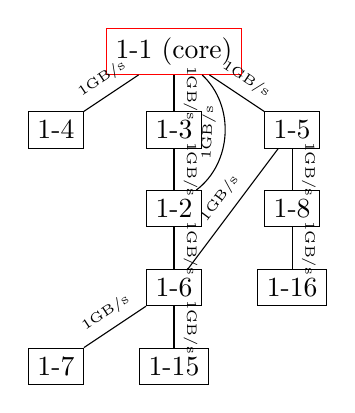
\begin{tikzpicture}
    \node[shape=rectangle,draw=red] (1-1) at (0,0) {1-1 (core)};
    \node[shape=rectangle,draw=black] (1-2) at (0,-2) {1-2};
    \node[shape=rectangle,draw=black] (1-3) at (0,-1) {1-3};
    \node[shape=rectangle,draw=black] (1-4) at (-1.5,-1) {1-4};
    \node[shape=rectangle,draw=black] (1-5) at (1.5,-1) {1-5};
    \node[shape=rectangle,draw=black] (1-6) at (0,-3) {1-6};
    \node[shape=rectangle,draw=black] (1-7) at (-1.5,-4) {1-7};
    \node[shape=rectangle,draw=black] (1-8) at (1.5,-2) {1-8};
    \node[shape=rectangle,draw=black] (1-15) at (0,-4) {1-15};
    \node[shape=rectangle,draw=black] (1-16) at (1.5,-3) {1-16};
    
    \path[-]	
    (1-1) edge node[sloped, anchor=center, above] {\tiny 1GB/s} (1-4) 
    (1-1) edge node[sloped, anchor=center, above] {\tiny 1GB/s} (1-3)
    (1-1) edge node[sloped, anchor=center, above] {\tiny 1GB/s} (1-5)
    (1-1) edge[bend left=50] node[sloped, anchor=center, above] {\tiny 1GB/s} (1-2)
    (1-2) edge node[sloped, anchor=center, above] {\tiny 1GB/s} (1-6)
    (1-3) edge node[sloped, anchor=center, above] {\tiny 1GB/s} (1-2)
    (1-5) edge node[sloped, anchor=center, above] {\tiny 1GB/s} (1-8)
    (1-5) edge node[sloped, anchor=center, above] {\tiny 1GB/s} (1-6)
    (1-6) edge node[sloped, anchor=center, above] {\tiny 1GB/s} (1-7)
    (1-6) edge node[sloped, anchor=center, above] {\tiny 1GB/s} (1-15)
    (1-8) edge node[sloped, anchor=center, above] {\tiny 1GB/s} (1-16)
    ;
    \end{tikzpicture}
    \caption{Example topology with annotated bandwidth}
    \label{fig:main:exampleTopology}
\end{figure}

When a new inspector is implemented inside an ISD, he has to construct the topology by periodically fetch the newest path requests. Because the topology remains static rather than constantly changing, the fetch rate can be high at the beginning and decrease to a normal value. For example, when the inspector is created, the fetch rate is 0.1 second and will decrease to 1.0 second of a few hours. 

\todo{Use work of ? with his buckets to get the values}

\subsection{Classify user}
This part will explain what a greedy user is and how to distinguish between a greedy and a normal user. It contain a definition for this work, which will later be used.

A greedy user is a user, who uses his network resources as the bandwidth in a selfish way and tries to maximize his personal benefit by using as much bandwidth as possible. He even may try to overuses his subscribed bandwidth or avoid the limits by using multi path communication.

An user may also be classified as a more greedy user than a fair user, when here is a congestion in the network and this user uses the most bandwidth. He may not be acting greedy in the first place, but he can be considered greedy in a global view.

Because of this we have to view two aspects which can classify a user as greedy. The first is the use of his resources. He can stay in the limit or he can overuse it. The second is if his activity causes a congestion.
\begin{table}[h]
    \centering
    \begin{tabular}{ r|c|c| }
        \multicolumn{1}{r}{}
        &  \multicolumn{1}{c}{no congestion}
        & \multicolumn{1}{c}{congestion} \\
        \cline{2-3}
        stays in limit & I & II \\
        \cline{2-3}
        overuses limit & III & IV \\
        \cline{2-3}
    \end{tabular}
    \caption{Different cases of a greedy user}
    \label{tab:classifyUser}    
\end{table}

\autoref{tab:classifyUser} shows these different four cases. The stays im limit or overuses limit means only the bandwidth usage of one connection between two ASes. An AS can have multiple connection to different ASes and can stay in his local limits.

\subsubsection{Case I - Fair user} \label{sub:main:detection:case1}
This user uses fewer bandwidth than he has subscribed to. There is also no congestion inside the network. In this case, there is no need to punish the user. They could use even more bandwidth, because it is currently underutilized and wasted.

\subsubsection{Case II - Global greedy user}
In this case there is a congestion inside the network. The currently used bandwidth is higher than the available. But there is no user who uses more bandwidth than he has subscribed to. Because of the missing culprit the punishment is not as easy as in case 4.

There is a need to find the most greedy user and try to convince him to use less resources for a better network experience for every user. The problem is, to find the most greedy user and to distinguish him from other user.

This can be done by using a clustering algorithm to find user with a similar behaviour. The cluster algorithm needs to find the outlier using more bandwidth than other. It also has to perform well with bigger sizes of elements, any $log(n^2)$ or worse runtime complexity is not sufficient. Because of using only the bandwidth as an attribute, it is possible to use algorithm based on arrays or lists of values, which results in simpler and more efficient algorithm.

The algorithm used for this work is the \textit{Jenks Natural Breaks} algorithm. \todo{Add good source}
%, Jenks Natural Breaks: https://www.ehdp.com/vitalnet/breaks-1.htm, http://wiki.objectvision.nl/index.php/Fisher\%27s_Natural_Breaks_Classification
It is applied to a sorted list of values and find good fitting ranges with also a rating value from 0 (worst fit) to 1 (perfect fit). Originally used for creating chloropleth maps, it can be used to divide the amount of users into two groups: fair user and user with high bandwidth usage. 

\todo{Explain the algorithm?}

If the GVF is higher than 0.8 we can assume, that the second range describes user who uses more bandwidth than the other. The member in this range can be considered as more greedy user than the other.


\todo{Add figure to display the issue}

\subsubsection{Case III - Overusing with no congestion}
This case occurs when there is no congestion, but an AS uses more bandwidth than it has subscribed for. For example, an AS has only a subscription for 1 GBit/s, but uses 1.2 GBit/s. The difference to case IV is, that beside overusing, there is no congestion.

On the one hand this behaviour can quickly lead to a congestion when everybody is doing it. On the other hand this behaviour utilizes the bandwidth in a better way, because the wasted bandwidth by not using it is lower.

The user can be clearly considered as greedy, but do not need to be punished immediately. A better way would be to tolerate a certain percentage of overuse and punish the user if he uses more than tolerated. The tolerance range would be 10\% without any problems. If the AS uses more than 110\% of its bandwidth the AS should be considered as a greedy user and receive a delayed punishment.

\todo{Add line graph to visualize this part}

\subsubsection{Case IV - Overuse resulted in a congestion}
This case is much more simpler than the other. If there is a congestion any user who overuses his bandwidth is considered a greedy user and have to receive immediately punishment to reduce or stop the congestion. 

\section{Next parts}
\begin{easylist}
    \MyListProperties
        ## Parameters of detection scheme
        ### Frequency
        ### Duration
        ### Sample size
        ## Security
        ### How to prevent lying AS
        ### How to prevent misusing the system(for dDos)
        # Punishment scheme
        ## Overview
        ## Level system for punishment (\textit{Flensburger system})
        ### \textit{Table of different levels and their punishments}
        ### How to get \"points\"
        ### Explain the levels
        ## Enforcement of punishment
        ### Describe responsibility (coreAS or coordinator?)
    \end{easylist}
\subfilebib % Makes bibliography available when compiling as subfile
\end{document}